% \documentclass[draftcls, journal, onecolumn]{IEEEtran}
% \documentclass[journal,draftcls,onecolumn,12pt,twoside]{IEEEtranTCOM}
\documentclass[journal]{IEEEtran}

%% Packages retained from the supplied journal template.
\usepackage{booktabs}
\usepackage{amsfonts}
\usepackage{placeins}
\usepackage{acronym}
\usepackage{amsmath}
\usepackage{tabularx}
\usepackage{stfloats}
\usepackage{siunitx}
\usepackage{amsmath,amssymb,amsfonts}
\usepackage{graphicx}
\usepackage{subcaption}
\captionsetup{compatibility=false}
\usepackage{setspace}
\usepackage{mathtools}
\usepackage{color}
\usepackage{array}
\usepackage[version=4]{mhchem}
\usepackage{float}
\usepackage{stmaryrd}
\usepackage{soul}
\usepackage{stackrel}
\usepackage{epstopdf}
\usepackage{url}
\usepackage{cite}
\usepackage{tikz}
\usetikzlibrary{automata,arrows,positioning,calc}
\usepackage{bigints}
\usepackage{threeparttable}
\usepackage{bbm}
\usepackage{dsfont}
\usepackage{pgfplots}\pgfplotsset{compat=1.18}
\usetikzlibrary{arrows.meta,positioning,angles,quotes,shadings,fit,shapes.geometric}

\newcolumntype{L}[1]{>{\raggedright\arraybackslash}m{#1}}
\newcolumntype{C}[1]{>{\centering\arraybackslash}m{#1}}
\acrodef{MRI}{magnetic resonance imaging}
\acrodef{T2W}{T2-weighted}
\acrodef{DWI}{diffusion-weighted imaging}
\acrodef{CNN}{convolutional neural network}
\acrodef{CVNN}{complex-valued neural network}
\acrodef{RVNN}{real-valued neural network}
\acrodef{PI-RADS}{Prostate Imaging Reporting and Data System}
\acrodef{FFT}{fast Fourier transform}
\acrodef{RSS}{root-sum-of-squares}
\acrodef{RMS}{root-mean-square}
\acrodef{BN}{batch normalization}
\acrodef{AUC}{area under the receiver operating characteristic curve}
\acrodef{ROC}{receiver operating characteristic}
\acrodef{AP}{average precision}
\acrodef{BCE}{binary cross entropy}
\acrodef{GRAPPA}{generalized autocalibrating partially parallel acquisitions}
\acrodef{ACS}{autocalibration signal}
\acrodef{CI}{confidence interval}
\acrodef{WL}{widely linear}


\begin{document}

\title{Complex-Valued Neural Networks for Prostate MRI Classification: A Parameter-Matched Factorial Study}

\author{Authors%
\thanks{Author list, affiliations, funding information, and corresponding-author details are placeholders in this first manuscript draft and should be finalized before submission.}}

\markboth{ASHRAF \MakeLowercase{et al.}: Complex-Valued Neural Networks for Prostate MRI Classification}%
{Ashraf \MakeLowercase{\emph{et al.}}}

\maketitle

\newcommand{\rev}[1]{\textcolor{red}{#1}}
\newcommand{\placeholderfig}[2]{%
\begin{figure}[t]
    \centering
    \fbox{\parbox[c][4.0cm][c]{0.91\linewidth}{\centering\small #1}}
    \caption{\small #2}
\end{figure}}

\begin{abstract}
Magnetic resonance data are acquired as complex-valued signals, yet diagnostic deep-learning pipelines commonly discard phase and operate on magnitude images. This work investigates whether retaining the native complex representation provides a measurable advantage for prostate MRI classification. Using a prepared four-coil subset of the public fastMRI Prostate T2-weighted data, we formulate slice-level binary classification of PI-RADS 3--5 versus PI-RADS 1--2 and compare a fixed real-valued magnitude CNN with parameter-matched complex-valued alternatives. The complex design is evaluated through a prespecified factorial experiment spanning image- and k-space inputs, three complex pooling operators, two normalization schemes, standard and widely-linear convolution, four activation functions, and five stream/interaction designs, yielding 480 complex configurations in addition to the real baseline. A technical pilot is separated from a four-seed confirmatory phase. The retained primary comparison is the paired test-AUC difference between a canonical complex model using magnitude-median pooling and the real baseline; all remaining factorial comparisons are treated as exploratory. \rev{[Insert final confirmatory mean test AUCs, paired $\Delta$AUC with interval, and win count after completion of the running experiments.] } The study is designed to distinguish the value of complex representation from simple increases in model capacity and to identify which complex-valued architectural choices are most relevant for MRI classification.
\end{abstract}

\begin{IEEEkeywords}
Complex-valued neural networks, magnetic resonance imaging, prostate MRI, fastMRI, k-space, phase information, medical image classification.
\end{IEEEkeywords}

\IEEEpeerreviewmaketitle
\acresetall

% =============================================================================
\section{Introduction}\label{sec:introduction}
% =============================================================================
\IEEEPARstart{M}{agnetic} resonance imaging is intrinsically complex-valued. The receiver coils measure oscillating electromagnetic signals whose discretized samples are represented by real and imaginary components in spatial-frequency space, or k-space. Image formation subsequently combines Fourier reconstruction, coil information, and magnitude operations into representations optimized for human interpretation. In most diagnostic machine-learning pipelines, the final input is consequently a real-valued magnitude image. This convention is natural from a clinical-imaging perspective, but it removes explicit phase information before the learning algorithm is given an opportunity to determine whether that information is useful for the task.

The distinction is relevant because magnitude and phase are not independent bookkeeping devices. A complex sample $z=a+\mathrm{i}b=r\mathrm{e}^{\mathrm{i}\phi}$ jointly represents amplitude $r$ and phase $\phi$. Operations in the complex domain therefore couple two real degrees of freedom through a structured algebra. A conventional real-valued network can in principle receive the real and imaginary components as independent channels and learn useful interactions, but its layers do not impose the multiplication rules, rotation structure, or phase relationships that are native to the data. A \ac{CVNN}, by contrast, implements these relationships directly through complex convolution and complex-aware nonlinearities and normalization. This inductive bias is attractive when the signal-generating process itself is naturally complex-valued.

Complex-valued deep learning is well established at the methodological level. Trabelsi \emph{et al.} developed practical complex convolution, normalization, initialization, and activation machinery for deep networks~\cite{Trabelsi2018DeepComplex}. In MRI, several studies have shown advantages of complex-valued processing for reconstruction and explicitly phase-dependent problems. Cole \emph{et al.} reported parameter-controlled comparisons in which complex networks improved accelerated MRI reconstruction and phase-focused applications~\cite{Cole2021ComplexMRI}, while Xiao \emph{et al.} demonstrated complex-valued learning for partial-Fourier recovery of both magnitude and phase~\cite{Xiao2022ComplexPartialFourier}. Virtue \emph{et al.} also explored complex-valued networks and phase-sensitive activations for MR fingerprinting~\cite{Virtue2017ComplexActivation}. These results make a strong case that complex-valued modeling can be useful when the target depends directly on signal phase or reconstruction fidelity. They do not, however, establish that the same advantage transfers to diagnostic classification, where labels are substantially farther from the acquisition physics.

The fastMRI project has enabled systematic study of learning from raw MR data by releasing raw k-space together with reconstructed images~\cite{Knoll2020fastMRI}. Its prostate extension provides biparametric prostate MRI, including T2-weighted and diffusion-weighted acquisitions, raw multi-coil data, reconstructions, and radiologist-assigned labels~\cite{Tibrewala2024FastMRIProstate}. The accompanying benchmark showed that conventional magnitude-image models can learn diagnostically relevant information from this dataset. This creates a useful controlled setting for a more specific question: when the same classification problem is approached with the native complex coil information, does preserving phase improve discrimination beyond what can be achieved from magnitude alone?

\subsection{Why Phase May Matter for Diagnostic Classification}
The diagnostic relevance of phase is less direct than its relevance for reconstruction, but there are several reasons not to discard it a priori. In a multi-coil acquisition, the measured complex signal is modulated by spatially varying coil sensitivities as well as by the underlying object. Magnitude combines part of this information into a nonnegative intensity representation, whereas the relative complex relationships between coils retain additional spatial structure. A discriminative model could exploit these relationships even when no individual phase map is itself visually interpretable as a diagnostic image.

A second consideration is that phase and magnitude respond differently to transformations and perturbations. If all coils are multiplied by a common phase factor $\mathrm{e}^{\mathrm{i}\alpha}$, magnitudes are unchanged and the diagnostic label should remain unchanged. A desirable complex representation can therefore be equivariant through feature extraction and invariant at the classification head. For a complex-linear map $f$ without phase-breaking nonlinearities,
\begin{align}
f(\mathrm{e}^{\mathrm{i}\alpha}z)
=\mathrm{e}^{\mathrm{i}\alpha}f(z).
\end{align}
If the final classifier depends on $|f(z)|$, this common rotation cancels. The implemented global-phase augmentation enforces the same task-level assumption even for configurations whose nonlinearities or normalization are not exactly equivariant. In this sense, the experiment probes not only whether phase is present, but also how strongly phase-consistent architectural constraints should be imposed.

A third consideration is statistical efficiency. Representing a complex tensor as independent real-valued channels leaves the network to learn the algebraic coupling between Cartesian components from data. A complex convolution hard-codes one particular coupling. This reduces freedom relative to an unrestricted real-linear map and can act as a structured regularizer when the assumption is appropriate. Widely-linear convolution relaxes that constraint by including the conjugate input. Comparing these alternatives at matched scalar parameter count therefore tests a continuum from stronger complex structure to greater real-linear flexibility.

At the same time, phase is a potential source of nuisance variation. Scanner-dependent offsets, motion, field inhomogeneity, and coil sensitivity can create reproducible phase patterns that are not biological markers. The phase-alignment and augmentation stages are therefore not cosmetic preprocessing. They define which phase degrees of freedom the model is allowed to use. We remove arbitrary global inter-coil offsets, preserve spatial phase variation inside the signal support, and randomize the remaining common global phase during training. The intended target is thus a representation that can exploit relative and spatial phase while remaining insensitive to an arbitrary overall rotation.

This distinction also motivates the magnitude-only baseline used here. The baseline represents the practical question faced by many imaging pipelines: should the complex acquisition be reduced to magnitude before diagnostic feature learning? A future information-matched control that supplies real and imaginary channels to a real network will be useful for distinguishing the value of phase information from the value of complex algebra itself. The present study first addresses the clinically common magnitude-versus-complex comparison under controlled model capacity.

Answering that question requires more than comparing one arbitrary real network with one arbitrary complex network. Complex architectures contain several design choices that can strongly change their behavior. Complex convolution may be strictly complex-linear or widely linear; normalization may preserve global phase equivariance or whiten real-imaginary covariance; nonlinearities may preserve phase, gate magnitude, or independently threshold the Cartesian components; pooling may select a complex sample by its magnitude, use a robust median-like selection, or average the complex values; and the network may process only a complex stream or combine complex and magnitude streams. If these factors are not controlled, an observed difference between a real and a complex model can be confounded by model capacity or by one implementation choice.

This work therefore treats complex-valued prostate MRI classification as a controlled factorial study. A fixed four-block real-valued CNN receiving coil magnitudes defines the reference model. Complex models are parameter matched to this baseline and vary along six prespecified architectural factors. The resulting grid contains 480 complex configurations. The experiment uses a technical pilot seed to verify the pipeline and four independent confirmatory seeds for the retained primary comparison. The pilot is excluded from confirmatory inference. The primary endpoint is the paired difference in held-out test \ac{AUC} between the canonical magnitude-median complex model and the real magnitude baseline. The remaining factorial comparisons are explicitly exploratory and are used to identify promising inductive biases rather than to support a large family of confirmatory claims.

The central hypothesis is that the complex representation provides useful information and structure beyond magnitude alone. Importantly, this hypothesis has two separable interpretations. The first is an \emph{information hypothesis}: phase carries signal components that correlate with the PI-RADS-derived classification target. The second is an \emph{inductive-bias hypothesis}: even when the information could theoretically be encoded in a real representation, complex operations may make the relevant relationships easier to learn with finite data. The factorial design cannot fully disentangle all causal mechanisms, but it can test whether the effect is robust to important complex-network choices and whether particular phase-aware operations are associated with performance gains.

The main contributions of this paper are as follows:
\begin{itemize}
    \item We formulate a controlled real-versus-complex prostate MRI classification study using four-coil T2-weighted fastMRI Prostate data and patient-disjoint train, validation, and test partitions.
    \item We implement a compact real magnitude CNN and a family of parameter-matched complex CNNs, keeping the trainable scalar parameter count within 1\% of the fixed real baseline.
    \item We evaluate a 480-configuration complex factorial grid covering input domain, pooling, normalization, convolution type, activation, and stream/interaction strategy, rather than drawing conclusions from a single complex architecture.
    \item We prespecify a confirmatory comparison between the real baseline and a canonical phase-preserving complex model using magnitude-median pooling, while treating the remainder of the grid as exploratory.
    \item We provide a reproducible evaluation protocol based on validation-AUC checkpoint selection, validation balanced-accuracy threshold selection, held-out test metrics, and paired seed-level comparisons.
\end{itemize}

The remainder of the paper is organized as follows. Section~\ref{sec:data} describes the dataset, labels, complex preprocessing, and classification formulation. Section~\ref{sec:models} defines the real and complex models and the individual complex-valued building blocks. Section~\ref{sec:design} presents the factorial experiment, training protocol, and statistical analysis. Section~\ref{sec:results} is structured for the confirmatory and exploratory results. Section~\ref{sec:discussion} discusses the interpretation, limitations, and implications of the study, and Section~\ref{sec:conclusion} concludes the paper.

% =============================================================================
\section{Dataset and Problem Formulation}\label{sec:data}
% =============================================================================
\subsection{fastMRI Prostate Dataset}
The fastMRI Prostate dataset extends the fastMRI resource to biparametric prostate MRI and includes raw k-space, reconstructed images, and clinical labels~\cite{Tibrewala2024FastMRIProstate}. The full release contains T2-weighted and diffusion-weighted acquisitions collected from a clinical population. The present experiments use the prepared T2-weighted subset available to the training pipeline. Each learning sample is one reconstructed axial slice represented by four selected complex-valued coil channels. The stored tensor has shape $4\times H\times W$ and is resized or prepared at $224\times224$ for the current classification experiment.

The classification target follows the slice-level PI-RADS labels supplied with the prostate dataset. PI-RADS is a standardized assessment system for prostate MRI~\cite{Turkbey2019PIRADSv21}. We define the positive class as PI-RADS 3--5 and the negative class as PI-RADS 1--2, matching the binary grouping used in the prepared manifest. This target should be interpreted as classification of slices with higher radiological suspicion rather than a direct histopathological diagnosis of prostate cancer. The distinction is important because the labels originate from imaging assessment and therefore inherit the uncertainty and task definition of PI-RADS itself.

Table~\ref{tab:cohort} summarizes the prepared cohort used by the current experiments. The dataset contains 8,225 slices from 270 patients. Patient identifiers are disjoint between training, validation, and test sets, preventing slices from a patient from appearing in more than one split. The class distribution is strongly imbalanced, with positive slices representing a small fraction of each partition. This imbalance motivates balanced sampling during training and the use of threshold-independent discrimination metrics for primary evaluation.

\begin{table}[t]
\centering
\caption{Prepared T2-weighted cohort used in the current experiment. Patient identifiers are disjoint across splits.}
\label{tab:cohort}
\scriptsize
\begin{tabular}{lrrrr}
\toprule
Split & Patients & Slices & PI-RADS 1--2 & PI-RADS 3--5 \\
\midrule
Training   & 189 & 5,672 & 5,373 & 299 \\
Validation & 41  & 1,308 & 1,223 & 85 \\
Test       & 40  & 1,245 & 1,182 & 63 \\
\midrule
Total      & 270 & 8,225 & 7,778 & 447 \\
\bottomrule
\end{tabular}
\end{table}

The full fastMRI Prostate release contains more subjects and slices than the prepared subset used here~\cite{Tibrewala2024FastMRIProstate}. The reduction is therefore a property of the present data-preparation pipeline and experimental cohort, not a description of the complete public dataset. For reproducibility, the experiment manifest records the sample path, patient identifier, binary label, split, and selected channels for every sample.

\subsection{Complex Coil Representation and Phase Alignment}
Let the four-coil complex image for a slice be
\begin{align}
\mathbf{x} &= [x_1,x_2,x_3,x_4], \\
x_c(u,v) &= a_c(u,v)+\mathrm{i}b_c(u,v)
           = r_c(u,v)\mathrm{e}^{\mathrm{i}\phi_c(u,v)},
\end{align}
where $c$ indexes the selected receiver coil. Coil phases can contain arbitrary global offsets that are unrelated to anatomy and may vary between acquisitions. Feeding such offsets directly to a phase-sensitive model can force the network to learn nuisance rotations and can obscure reproducible inter-coil phase relationships. The preprocessing therefore aligns the coil phases before model input.

A signal support is first estimated from the \ac{RSS} magnitude. The implementation uses the 99th percentile of the signal magnitude as a robust scale and defines a foreground support relative to this scale. The first selected coil acts as the phase reference. A global phase is removed from the reference coil, after which each remaining coil is aligned to the reference through the cross-phase within the foreground support. Background values outside the estimated support are set to zero. This procedure removes arbitrary inter-coil offsets while retaining spatially varying phase structure inside the object.

After phase alignment, every sample receives one shared robust magnitude scale. If $q_{0.99}$ denotes the sample's 99th percentile magnitude across the complex tensor, the scaled input is
\begin{align}
\tilde{\mathbf{x}} = \frac{\mathbf{x}}{q_{0.99}+\epsilon}.
\end{align}
The same scalar divides real and imaginary components and all four coils. Consequently, relative coil magnitudes and complex phase are preserved. Shared scaling is particularly important for the real-versus-complex comparison: independently normalizing real and imaginary components would change the geometry of the complex signal and introduce a preprocessing difference not present in the magnitude baseline.

\begin{figure*}[t]
\centering
\fbox{\parbox[c][4.2cm][c]{0.92\textwidth}{\centering\small
\textbf{DATA FIGURE PLACEHOLDER}\\[0.65em]
Recommended final figure: one representative slice with the four coil magnitudes, four aligned phase maps inside the foreground mask, and corresponding centered log-magnitude k-space views.\\[0.65em]
This figure should be generated from a non-identifying sample in the prepared dataset using exactly the preprocessing employed by the data loader.}}
\caption{\small Recommended visualization of the model inputs after complex phase alignment. The final version should show how magnitude, spatial phase, and Fourier-domain structure differ across the four selected receiver coils.}
\label{fig:complexinput}
\end{figure*}

\subsection{Image-Space and k-Space Inputs}
The factorial experiment includes two input domains for complex models. In the image-domain condition, the phase-aligned complex coil images are used directly. In the k-space condition, each complex coil image is transformed with a centered orthonormal two-dimensional Fourier transform,
\begin{align}
X_c(k_x,k_y)
= \mathcal{F}_{\mathrm{c}}\{x_c(u,v)\},
\end{align}
implemented using an inverse shift, a two-dimensional \ac{FFT} with orthonormal normalization, and a final center shift. The resulting k-space tensor is then robustly scaled using the same shared-magnitude principle.

The k-space arm is included to test whether a complex network benefits from operating closer to the acquisition domain. It is not equivalent to training on the raw, unprocessed fastMRI acquisition in every respect: the current prepared samples originate from the experiment's four-coil complex image representation and are transformed to k-space within the data loader. Thus, conclusions should be phrased as an image-domain versus Fourier-domain representation comparison under the current preprocessing, rather than as a comparison between clinical reconstruction and untouched scanner raw data.

The real baseline receives magnitude only,
\begin{align}
\mathbf{x}_{\mathrm{real}} = |\tilde{\mathbf{x}}|\in\mathbb{R}^{4\times H\times W}.
\end{align}
This choice makes the reference model representative of the common practice of discarding phase while preserving coil-specific magnitude channels. The factorial grid does not include a separate real-valued k-space baseline. Accordingly, comparisons between image and k-space are made within the complex family; the prespecified real-versus-complex primary comparison uses the canonical image-domain complex model.

\subsection{Global-Phase Augmentation}
Complex models are augmented during training with a random global phase rotation,
\begin{align}
\tilde{\mathbf{x}}' = \tilde{\mathbf{x}}\,\mathrm{e}^{\mathrm{i}\theta},
\qquad \theta\sim\mathcal{U}[-\pi,\pi].
\label{eq:globalphase}
\end{align}
This augmentation leaves all magnitudes unchanged and therefore preserves the real baseline representation, while explicitly discouraging complex models from associating the target with an arbitrary absolute global phase. Validation and test data are not phase augmented. Conceptually, Eq.~\eqref{eq:globalphase} encodes the assumption that the label should be invariant to a common rotation of all complex channels, while relative and spatial phase patterns may remain informative.

\subsection{Classification Task}
For a slice input $\mathbf{x}$ and binary target $y\in\{0,1\}$, the model produces a scalar logit $s_\theta(\mathbf{x})$. The probability estimate is
\begin{align}
\hat p_\theta(y=1\mid\mathbf{x})
= \sigma(s_\theta(\mathbf{x})),
\end{align}
where $\sigma(\cdot)$ is the logistic sigmoid. Training minimizes unweighted binary cross entropy at the sample level. Class imbalance is handled in the sampling distribution rather than by changing the loss: the training loader uses a weighted random sampler with equal total sampling mass assigned to the positive and negative classes. Therefore, rare positive slices are sampled more frequently while the validation and test distributions remain unchanged.

The primary performance measure is test \ac{AUC}, which evaluates ranking independently of a fixed classification threshold. For threshold-dependent metrics, a threshold is selected on the validation set by maximizing balanced accuracy and is then frozen before test evaluation. This separation avoids choosing a test threshold after observing the held-out labels.

\begin{figure*}[t]
\centering
\resizebox{0.98\textwidth}{!}{%
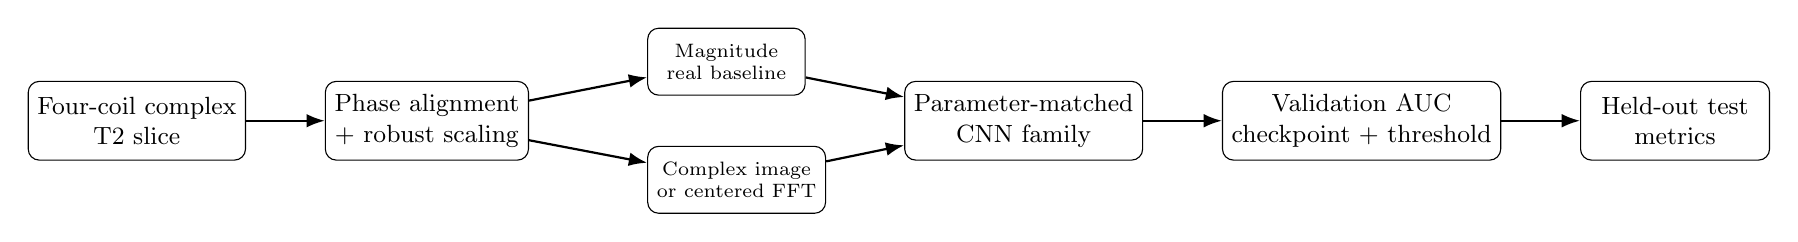
\begin{tikzpicture}[
    node distance=1.15cm and 1.0cm,
    block/.style={draw,rounded corners,minimum height=1.0cm,minimum width=2.4cm,align=center,font=\small},
    smallblock/.style={draw,rounded corners,minimum height=0.85cm,minimum width=2.0cm,align=center,font=\scriptsize},
    arrow/.style={-Latex,thick}
]
\node[block] (data) {Four-coil complex\\T2 slice};
\node[block,right=of data] (prep) {Phase alignment\\+ robust scaling};
\node[smallblock,right=1.5cm of prep,yshift=0.75cm] (real) {Magnitude\\real baseline};
\node[smallblock,right=1.5cm of prep,yshift=-0.75cm] (complex) {Complex image\\or centered FFT};
\node[block,right=1.25cm of real,yshift=-0.75cm] (models) {Parameter-matched\\CNN family};
\node[block,right=of models] (sel) {Validation AUC\\checkpoint + threshold};
\node[block,right=of sel] (test) {Held-out test\\metrics};
\draw[arrow] (data) -- (prep);
\draw[arrow] (prep) -- (real);
\draw[arrow] (prep) -- (complex);
\draw[arrow] (real) -- (models);
\draw[arrow] (complex) -- (models);
\draw[arrow] (models) -- (sel);
\draw[arrow] (sel) -- (test);
\end{tikzpicture}}
\caption{\small Overview of the experimental pipeline. The real baseline receives the four coil magnitudes. Complex models retain real-imaginary structure and are evaluated in image or Fourier domain. Data splits are patient disjoint, and model/threshold selection uses validation data only.}
\label{fig:pipeline}
\end{figure*}

% =============================================================================
\section{Complex-Valued Classification Models}\label{sec:models}
% =============================================================================
\subsection{Parameter-Matched Real-Valued Baseline}
The reference network is a compact four-stage \ac{CNN} receiving the four coil magnitudes. Its channel widths are
\begin{align}
45 \rightarrow 91 \rightarrow 181 \rightarrow 272.
\end{align}
Each stage contains two $3\times3$ real convolutions, each followed by batch normalization and a SiLU nonlinearity. A $2\times2$ max-pooling operation follows each of the first three stages. After the fourth stage, adaptive global average pooling reduces the feature maps to a channel vector. Dropout with probability $0.2$ is applied immediately before a one-unit linear classification head.

This architecture contains 1,685,890 trainable scalar parameters. It is deliberately smaller than common large image-classification backbones. The goal of the study is not to maximize benchmark performance through scale, but to compare representational choices under closely controlled capacity. The real model therefore establishes a fixed parameter budget against which every complex configuration is matched.

\subsection{Standard Complex Convolution}
For an input $z=x_r+\mathrm{i}x_i$ and complex kernel $W=W_r+\mathrm{i}W_i$, standard complex convolution is implemented with real convolutions as
\begin{align}
W*z
&=(W_r*x_r-W_i*x_i) \\
&\quad+\mathrm{i}(W_r*x_i+W_i*x_r).
\label{eq:complexconv}
\end{align}
Unlike treating $x_r$ and $x_i$ as unrelated feature channels, Eq.~\eqref{eq:complexconv} ties the real-imaginary interactions according to complex multiplication. A common complex rotation of the input therefore propagates in a structured way through a sequence of complex-linear layers. This is one of the principal inductive biases under investigation.

The canonical complex network uses channel widths
\begin{align}
32 \rightarrow 64 \rightarrow 128 \rightarrow 192,
\end{align}
with two complex $3\times3$ convolutions per stage. For the canonical RMSNorm/standard-convolution/complex-only configuration these widths produce 1,681,473 trainable scalar parameters, within 1\% of the real baseline. Architectures that introduce additional convolutional weights, such as widely-linear or dual-stream variants, use automatically selected channel widths so that the same parameter-matching criterion is satisfied.

\subsection{Widely-Linear Complex Convolution}
Strict complex linearity may be unnecessarily restrictive for signals that are not circularly symmetric in the complex plane. Widely-linear estimation augments the complex input with its conjugate and has a long history in complex signal processing~\cite{Picinbono1995WidelyLinear}. The implemented layer has the form
\begin{align}
y = W_1*z + W_2*z^*,
\label{eq:wl}
\end{align}
where $z^*$ denotes complex conjugation. Equation~\eqref{eq:wl} can represent a broader family of real-linear transformations than standard complex convolution, at the cost of additional weights. Parameter matching therefore narrows the corresponding channel widths to keep scalar model capacity comparable to the real baseline.

The factorial comparison between standard and widely-linear convolution tests whether strict complex structure is beneficial for the present MRI task or whether the additional flexibility of conjugate interactions improves discrimination. A gain from widely-linear convolution would suggest that the useful relationships are complex-valued but not well modeled by strictly complex-linear transformations alone.

\subsection{Complex Normalization}
Two normalization schemes are evaluated. The first is complex RMS normalization. For a feature channel $z$, the layer estimates its mean squared complex magnitude and rescales the channel by
\begin{align}
\operatorname{RMSNorm}(z)
= \frac{z}{\sqrt{\mathbb{E}|z|^2+\epsilon}}\,g,
\end{align}
with learnable real gain $g$. Since the normalization depends on magnitude rather than absolute phase, it is compatible with global phase rotations.

The second alternative is complex batch normalization based on whitening the real-imaginary pair. Let $\mu_r$ and $\mu_i$ denote batch means and let
\begin{align}
\mathbf{V}=
\begin{bmatrix}
V_{rr} & V_{ri}\\
V_{ri} & V_{ii}
\end{bmatrix}
\end{align}
be the $2\times2$ covariance of the Cartesian components for a channel. Complex batch normalization applies an inverse square-root transform to approximately whiten the pair, followed by a learnable affine transformation. This approach follows the general complex-normalization framework of Trabelsi \emph{et al.}~\cite{Trabelsi2018DeepComplex}. It can normalize correlated real and imaginary components more completely than RMS scaling, but it introduces batch-statistics dependence and a less direct phase-equivariant interpretation.

\subsection{Complex Activation Functions}
Four activation functions are included because nonlinearity is one of the central unresolved design choices in complex networks.

\subsubsection{modReLU}
The canonical activation is modReLU, originally introduced for unitary recurrent networks~\cite{Arjovsky2016Unitary}. For $z\neq0$,
\begin{align}
\operatorname{modReLU}(z)
= z\frac{\operatorname{ReLU}(|z|+b)}{|z|+\epsilon},
\label{eq:modrelu}
\end{align}
where $b$ is learnable. The operation gates magnitude while preserving the phase of active units. This property makes it a natural baseline when one wants the nonlinear network to maintain phase equivariance as far as possible.

\subsubsection{Magnitude-gated SiLU}
The magnitude-gated SiLU variant multiplies the complex activation by a sigmoid gate derived from its magnitude,
\begin{align}
\operatorname{MagSiLU}(z)
= z\,\sigma\left(a(|z|-b)\right),
\end{align}
with learnable parameters controlling the gate. As with modReLU, the complex direction of $z$ is unchanged while its amplitude is modulated. Its smoother gate may improve optimization relative to a rectified magnitude threshold.

\subsubsection{CReLU}
The Cartesian ReLU applies conventional ReLU independently to the two components,
\begin{align}
\operatorname{CReLU}(z)
= \operatorname{ReLU}(\Re z)
+\mathrm{i}\operatorname{ReLU}(\Im z).
\end{align}
This activation is simple and expressive but does not preserve a common phase rotation. It therefore provides a useful contrast: if CReLU performs well, strict phase equivariance may not be necessary even when complex input is retained.

\subsubsection{Cardioid}
The cardioid activation uses the phase angle to scale the complex value,
\begin{align}
\operatorname{Cardioid}(z)
= \frac{1}{2}\left(1+\cos(\angle z)\right)z.
\end{align}
Phase-dependent complex activations have previously been explored in MRI applications~\cite{Virtue2017ComplexActivation}. In the present grid, the cardioid condition tests whether explicitly phase-selective gating improves classification over phase-preserving magnitude gates.

\subsection{Complex Pooling}
Downsampling complex-valued feature maps requires a definition of order or aggregation because complex numbers do not have a natural total ordering. Three alternatives are implemented.

\textit{Magnitude max pooling} identifies the element of each $2\times2$ window with the largest magnitude and returns the corresponding full complex value. Phase is therefore retained for the selected unit. \textit{Magnitude median pooling} ranks the four elements by magnitude and returns an observed complex activation at the median rank. This operation is intended to reduce sensitivity to isolated high-amplitude activations while still returning an actual complex sample rather than manufacturing a phase through averaging. For an even four-element window, the implementation uses the lower median rank. \textit{Complex average pooling} averages real and imaginary components over the window, equivalent to averaging the complex values directly.

The canonical primary complex model uses magnitude-median pooling. This choice was retained before the confirmatory phase and is not selected after inspecting confirmatory test performance. The max and average variants remain important ablations because pooling can determine how localized phase patterns survive spatial downsampling.

\subsection{Single- and Dual-Stream Feature Extraction}
The complex-only architecture contains four complex convolutional blocks with three intermediate pooling operations. After the third block, an optional holographic interaction module can be inserted. The final complex feature map is adaptively pooled after converting it to magnitude, and a real-valued linear head produces the binary logit. Thus, complex information is preserved throughout convolutional feature extraction and converted to a real invariant representation only near the classifier.

The dual-stream architecture processes both a real magnitude stream and a complex stream. The real branch uses conventional real-valued convolutional blocks, while the complex branch uses the selected complex operations. At the output, pooled real features are concatenated with magnitudes of the pooled complex features before classification. This design tests whether magnitude and phase-aware features are complementary rather than mutually exclusive representations.

Three interaction choices are used in the dual stream. With \textit{none}, the branches are independent until final fusion. With \textit{modulus gate}, the magnitude of the complex branch is transformed into a sigmoid spatial gate that modulates the real branch. With \textit{holographic interaction}, the complex branch contains an interference-aware attention operation. Complex-only models support either no interaction or holographic interaction; modulus gating is undefined without a real branch and is therefore excluded from that stream type.

\subsection{Interference-Aware Holographic Interaction}
The holographic module uses complex query, key, and value projections. For query $q_i$ and key $k_j$ with embedding dimension $d$, the similarity component is the real part of the Hermitian inner product,
\begin{align}
s_{ij}^{(H)}
= \frac{\Re\{q_i k_j^H\}}{\sqrt{d}}.
\end{align}
The implementation additionally penalizes squared distance in the complex plane,
\begin{align}
s_{ij}=s_{ij}^{(H)}
-\gamma\frac{\|q_i-k_j\|_2^2}{d},
\label{eq:holo}
\end{align}
with $\gamma=1$ in the current experiment. Softmax-normalized scores aggregate the complex values, followed by a residual connection and complex normalization. The module is intended to make constructive versus destructive complex similarity explicit, but its value for MRI classification is an exploratory question rather than an assumption of the study.

\begin{figure*}[t]
\centering
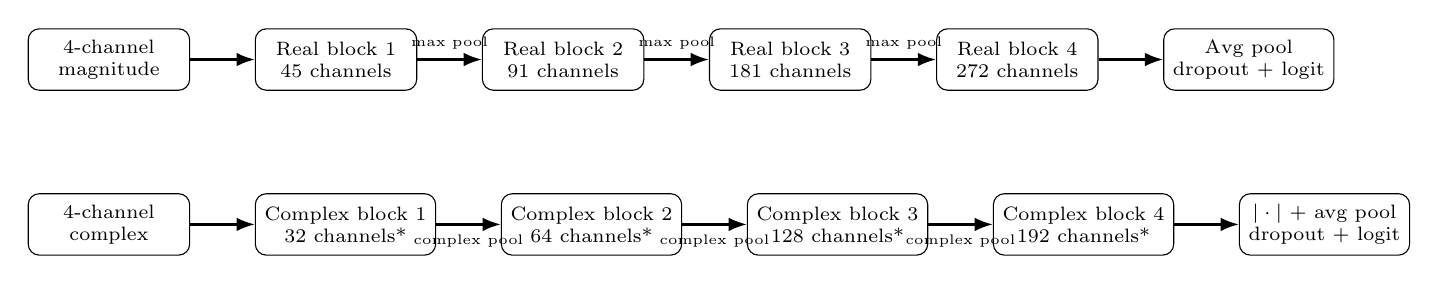
\begin{tikzpicture}[
node distance=0.72cm and 0.82cm,
blk/.style={draw,rounded corners,minimum width=2.05cm,minimum height=0.78cm,align=center,font=\scriptsize},
arr/.style={-Latex,thick}
]
\node[blk] (rin) {4-channel\\magnitude};
\node[blk,right=of rin] (rb1) {Real block 1\\45 channels};
\node[blk,right=of rb1] (rb2) {Real block 2\\91 channels};
\node[blk,right=of rb2] (rb3) {Real block 3\\181 channels};
\node[blk,right=of rb3] (rb4) {Real block 4\\272 channels};
\node[blk,right=of rb4] (rhead) {Avg pool\\dropout + logit};
\draw[arr] (rin)--(rb1); \draw[arr] (rb1)--node[above,font=\tiny]{max pool}(rb2); \draw[arr] (rb2)--node[above,font=\tiny]{max pool}(rb3); \draw[arr] (rb3)--node[above,font=\tiny]{max pool}(rb4); \draw[arr] (rb4)--(rhead);

\node[blk,below=1.3cm of rin] (cin) {4-channel\\complex};
\node[blk,right=of cin] (cb1) {Complex block 1\\32 channels*};
\node[blk,right=of cb1] (cb2) {Complex block 2\\64 channels*};
\node[blk,right=of cb2] (cb3) {Complex block 3\\128 channels*};
\node[blk,right=of cb3] (cb4) {Complex block 4\\192 channels*};
\node[blk,right=of cb4] (chead) {$|\cdot|$ + avg pool\\dropout + logit};
\draw[arr] (cin)--(cb1); \draw[arr] (cb1)--node[below,font=\tiny]{complex pool}(cb2); \draw[arr] (cb2)--node[below,font=\tiny]{complex pool}(cb3); \draw[arr] (cb3)--node[below,font=\tiny]{complex pool}(cb4); \draw[arr] (cb4)--(chead);
\end{tikzpicture}
\caption{\small Real baseline (top) and canonical complex-only architecture (bottom). Each block contains two $3\times3$ convolutions with the corresponding normalization and activation. The starred complex widths are the canonical standard-convolution widths; variants with extra operators are automatically narrowed to remain within 1\% of the real baseline's 1,685,890 trainable scalar parameters.}
\label{fig:architecture}
\end{figure*}

\begin{table*}[t]
\centering
\caption{Representative architecture definitions and parameter-budget role. Exact widths for noncanonical factorial variants are recorded per run after automatic parameter matching.}
\label{tab:architectures}
\scriptsize
\begin{tabularx}{\textwidth}{L{3.0cm}L{3.2cm}L{2.8cm}L{2.5cm}X}
\toprule
Model & Input / stream & Canonical widths & Trainable scalars & Main distinction \\
\midrule
Real baseline & 4 magnitude channels & 45/91/181/272 & 1,685,890 & Real conv + BatchNorm + SiLU + max pool \\
Canonical complex & 4 complex channels, complex-only & 32/64/128/192 & 1,681,473 & Standard complex conv + RMSNorm + modReLU; pooling varied \\
Widely-linear variants & Complex-only or dual & automatically matched & within 1\% of real & Adds $z^*$ pathway; widths reduced to offset additional kernels \\
Dual-stream variants & Magnitude + complex & automatically matched & within 1\% of real & Parallel real/complex feature extraction with optional interaction \\
\bottomrule
\end{tabularx}
\end{table*}

\begin{table*}[t]
\centering
\caption{Factors in the complex-valued factorial grid. Their Cartesian product contains 480 valid complex configurations.}
\label{tab:grid}
\scriptsize
\begin{tabularx}{\textwidth}{L{2.9cm}L{4.2cm}X}
\toprule
Factor & Levels & Intended question \\
\midrule
Input domain & Image; k-space & Does the representation closer to Fourier/acquisition space improve complex learning? \\
Pooling & Magnitude max; magnitude median; complex average & Which downsampling rule best preserves useful complex structure? \\
Normalization & Complex RMSNorm; complex BatchNorm & Is phase-compatible power scaling or real-imaginary whitening more effective? \\
Convolution & Standard; widely linear & Is strict complex linearity sufficient, or are conjugate interactions beneficial? \\
Activation & modReLU; magnitude-gated SiLU; CReLU; cardioid & Are phase-preserving, Cartesian, or phase-selective nonlinearities preferable? \\
Streams/interaction & Complex-only/none; complex-only/holographic; dual/none; dual/modulus-gate; dual/holographic & Does magnitude provide a complementary stream, and do explicit cross-feature interactions help? \\
\bottomrule
\end{tabularx}
\end{table*}

% =============================================================================
\section{Experimental Design}\label{sec:design}
% =============================================================================
\subsection{Prespecified Factorial Grid}
The experiment contains one fixed real baseline and the 480 complex configurations defined in Table~\ref{tab:grid}. The product is
\begin{align}
2\times3\times2\times2\times4\times5=480.
\end{align}
The grid is exhaustive over the implemented factor levels, with the sole structural exclusion that a modulus gate requires a real magnitude branch and is therefore not paired with a complex-only stream. Stable experiment keys identify the three original canonical pooling models: \texttt{complex\_max}, \texttt{complex\_median}, and \texttt{complex\_average}. All other keys encode the six factor settings so that run identity can be recovered directly from the output files.

The parameter count of the real model is held fixed. For every complex architecture, channel widths are treated as a dependent design variable. A width-selection routine searches channel scalings and records the exact widths and scalar parameter count in the run configuration. A complex model is accepted when its parameter count is within 1\% of the real baseline. This is essential because a naively implemented complex layer contains multiple real-valued kernels; without matching, apparent benefits could be explained simply by increased parameter count.

\subsection{Pilot and Confirmatory Phases}
The experiment is divided into two phases. The technical pilot uses random seed 10383 and runs all 481 models. Its purpose is to expose implementation failures, assess optimization behavior, and verify that all grid configurations can execute under the cluster workflow. The pilot is not included in confirmatory summaries.

The confirmatory phase uses four prespecified seeds: 24001, 24002, 24003, and 24004. Each seed runs the real baseline and all 480 complex configurations. This yields 1,924 confirmatory training tasks and 2,405 tasks when the pilot is included. Runs for each seed use identical data partitions and training hyperparameters; only stochastic initialization, sampling order, augmentation, and other seed-dependent training randomness change.

The separation between pilot and confirmatory seeds limits one common source of optimistic bias. Architectural or implementation decisions informed by the pilot can still influence the final system, but the primary numerical comparison is computed only on unseen confirmatory training seeds. The test set itself remains the same across seeds, making the analysis paired: for every seed, the real and complex models are evaluated on identical held-out samples.

\subsection{Analysis Hierarchy and Research Questions}
The factorial experiment is intentionally broader than the inferential scope of the paper. To avoid conflating model exploration with confirmation, we define a hierarchy of research questions before viewing the completed confirmatory summary. The first question is whether the canonical complex model improves test discrimination relative to the magnitude-only real baseline. This is the only comparison assigned a confirmatory statistical test. The second question is whether the canonical pooling variants show a stable ordering. The remaining questions concern architectural associations across the factorial grid and are descriptive.

This hierarchy is summarized in Table~\ref{tab:hypotheses}. It also determines the order of presentation in Section~\ref{sec:results}. The primary comparison is shown before any ranking of the 480-model grid. This prevents a post hoc best-performing configuration from replacing the prespecified model in the main claim. If a noncanonical configuration substantially outperforms both the real baseline and the canonical complex model, it is reported as an exploratory discovery and proposed for independent confirmation rather than retrospectively promoted to the primary endpoint.

A second reason for the hierarchy is that the factorial factors answer different types of questions. Input domain and stream structure change the representation available to the network; convolution, normalization, and activation alter the complex algebra and invariances; pooling changes how local complex features are spatially compressed. Their effects can interact strongly. For example, an activation that works well with RMSNorm may behave differently with covariance-whitening BatchNorm, and widely-linear convolution may reduce the value of a dual magnitude stream. Therefore, factor-level averages are used as summaries of the explored design space, not as an assumption of independent additive effects.

The experiment also distinguishes performance from optimization robustness. For each configuration, the four confirmatory seeds provide a small empirical distribution of outcomes under training stochasticity. A model with a high average AUC but large seed dispersion is less attractive for follow-up than a similarly performing model with stable paired gains. Accordingly, the eventual exploratory ranking should report both mean discrimination and consistency. This is especially important in the present class-imbalanced setting, where optimization noise can produce materially different minority-class decision boundaries even with fixed patient splits.

Finally, the analysis hierarchy constrains the language used in the conclusion. The confirmatory result can support a statement specifically about the canonical complex-versus-real comparison. Factorial observations can support statements such as ``the strongest configurations tended to use...'' or ``performance was higher on average for...'', but should not be presented as independently confirmed effects. This separation keeps the large experiment scientifically useful without converting an architecture search into an uncontrolled multiple-testing exercise.

\begin{table*}[t]
\centering
\caption{Prespecified hierarchy for interpreting the completed experiment.}
\label{tab:hypotheses}
\scriptsize
\begin{tabularx}{\textwidth}{L{1.5cm}L{5.0cm}L{4.1cm}X}
\toprule
Level & Research question & Comparison / summary & Intended interpretation \\
\midrule
Primary & Does the canonical phase-preserving complex model improve discrimination over magnitude-only learning? & \texttt{complex\_median} versus \texttt{real}, paired across four confirmatory seeds & Confirmatory effect size and consistency; exact sign-flip reported only here \\
Secondary descriptive & Is magnitude-median pooling preferable within the otherwise fixed canonical complex architecture? & \texttt{complex\_max}, \texttt{complex\_median}, \texttt{complex\_average} & Controlled pooling ablation; not a second confirmatory family \\
Exploratory & Which complex design factors are associated with higher AUC? & Marginal and stratified summaries of 480 configurations & Architectural hypothesis generation \\
Exploratory & Do explicit magnitude and complex streams provide complementary information? & Five stream/interaction levels & Representation/interaction hypothesis generation \\
Follow-up & Does a discovered configuration generalize beyond this experiment? & Independent split or external cohort & Required before elevating an exploratory winner to a new primary model \\
\bottomrule
\end{tabularx}
\end{table*}

\subsection{Optimization and Model Selection}
Training uses AdamW~\cite{Loshchilov2019AdamW} with learning rate $10^{-3}$ and weight decay $10^{-4}$. The maximum number of epochs is 100. Mini-batch size is 8 with four gradient-accumulation steps, giving an effective optimization batch of 32 samples. The loss is unweighted \ac{BCE} with logits. As described in Section~\ref{sec:data}, a weighted random sampler approximately balances positive and negative sampling mass during training.

Early stopping patience is eight epochs. Checkpoint selection is based on validation AUC; if the AUC is undefined in an exceptional validation state, validation loss provides a fallback ordering. After the best checkpoint is restored, the classification threshold is optimized on the validation set for balanced accuracy. That threshold is then applied unchanged to the test set. No test metric is used to choose the checkpoint, hyperparameters, model threshold, or primary complex architecture.

The real network and all complex networks use dropout probability 0.2 immediately before their final classifier. The current complex augmentation is the global phase rotation in Eq.~\eqref{eq:globalphase}; the training code does not apply the geometric rotation/translation/flip augmentation stated in an earlier manuscript draft. Keeping the manuscript synchronized with the implementation is particularly important here because spatial augmentation can alter the effective invariances being tested.

\subsection{Evaluation Metrics}
For every model and seed, the evaluation pipeline records accuracy, balanced accuracy, sensitivity, specificity, precision, F1 score, AUC, and average precision. Given the strong class imbalance, ordinary accuracy is not emphasized. AUC is the primary threshold-independent metric, while average precision is included because it is sensitive to performance in the positive minority class. Sensitivity and specificity use the validation-selected threshold and are reported to expose clinically relevant tradeoffs hidden by a single scalar discrimination metric.

For a model $m$ and confirmatory seed $s$, denote the test AUC by $A_{m,s}$. The prespecified primary effect is
\begin{align}
\Delta_s
= A_{\mathrm{complex\_median},s}
- A_{\mathrm{real},s}.
\label{eq:delta}
\end{align}
The primary summary reports the mean paired difference $\bar\Delta$, the four individual seed differences, a 10,000-resample percentile interval formed by resampling the seed-level paired differences, and the number of wins and ties. An exact paired sign-flip test is reserved for this primary endpoint. For all other complex configurations, analogous paired differences and intervals are reported descriptively without expanding the confirmatory hypothesis family.

With only four confirmatory seed pairs, formal seed-level inference is necessarily coarse. There are only $2^4=16$ possible sign assignments. Even if all four differences have the same nonzero sign and the observed statistic is maximally extreme, a conventional two-sided exact sign-flip calculation cannot attain a $p$-value below $2/16=0.125$. Consequently, the sign-flip result is interpreted as a consistency check rather than as a realistic route to $p<0.05$. The magnitude of the paired AUC difference, its stability across seeds, and patient-level uncertainty analyses are more informative for the eventual paper.

\subsection{Exploratory Factor Analysis}
The full 480-model grid is used to examine which complex architectural choices are associated with stronger performance. For each configuration $m$, paired test-AUC deltas relative to the real baseline are computed across confirmatory seeds. Configurations can then be ranked by mean AUC or mean paired delta. Factor-level summaries aggregate performance over all configurations sharing a level, for example standard versus widely-linear convolution or image versus k-space input.

These summaries are exploratory because the same held-out test set contributes to a large number of comparisons. The grid is designed for hypothesis generation and architectural understanding, not for declaring 480 independent discoveries. The eventual Results section should therefore report effect patterns, rank stability, and a limited number of representative configurations rather than emphasize the single numerically best run. If a configuration discovered through this grid is proposed as a new primary model, it should be evaluated in a subsequent independent experiment or external dataset.

\subsection{Reproducibility and Experiment Outputs}
Each run writes its resolved configuration, exact trainable parameter count, metrics, and completion status. The aggregation stage produces seed-level metrics, model summaries, paired deltas, paired summaries, and metadata describing whether all phase-two runs completed. Failed attempts are retained instead of overwritten, allowing errors to be traced without silently replacing unsuccessful runs. The cluster launcher also records the model grid and submission provenance.

The code architecture is particularly useful for manuscript reproducibility because every named factor in Table~\ref{tab:grid} maps to an explicit model option. Once the running experiment is complete, the numerical tables in Section~\ref{sec:results} can be populated directly from the generated CSV summaries rather than manually transcribing individual runs.

\begin{table}[t]
\centering
\caption{Fixed training and evaluation protocol.}
\label{tab:training}
\scriptsize
\begin{tabular}{ll}
\toprule
Setting & Value \\
\midrule
Optimizer & AdamW \\
Learning rate & $10^{-3}$ \\
Weight decay & $10^{-4}$ \\
Maximum epochs & 100 \\
Batch size & 8 \\
Gradient accumulation & 4 \\
Effective batch size & 32 \\
Early-stopping patience & 8 epochs \\
Checkpoint criterion & Validation AUC \\
Training imbalance control & Weighted random sampler \\
Loss & BCE with logits \\
Threshold selection & Max. validation balanced accuracy \\
Dropout before classifier & 0.2 \\
Pilot seed & 10383 \\
Confirmatory seeds & 24001--24004 \\
Primary endpoint & Paired test-AUC difference \\
\bottomrule
\end{tabular}
\end{table}

\begin{figure*}[t]
\centering
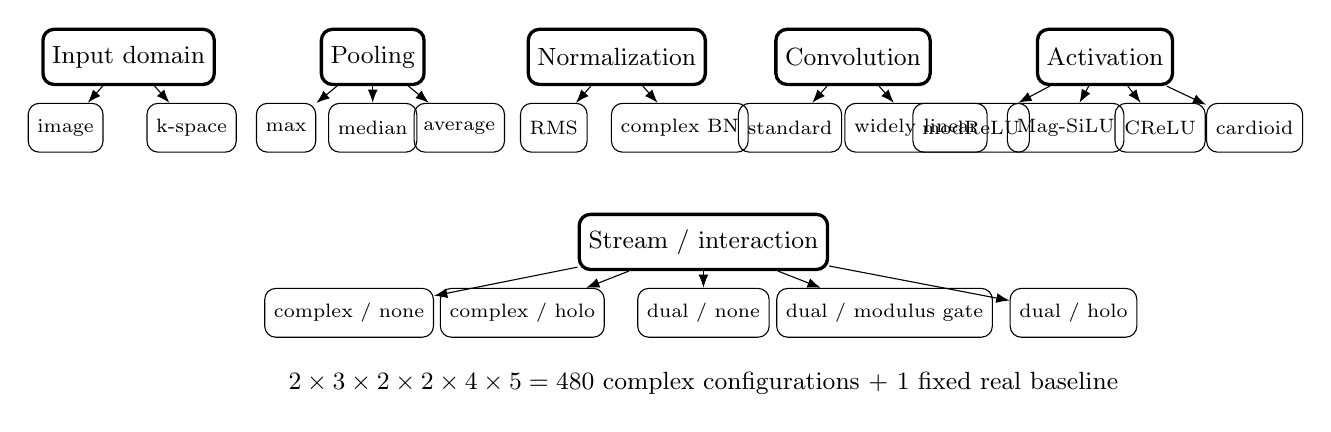
\begin{tikzpicture}[
    level/.style={draw,rounded corners,minimum height=0.62cm,align=center,font=\scriptsize},
    factor/.style={draw,very thick,rounded corners,minimum height=0.7cm,align=center,font=\small},
    arr/.style={-Latex}
]
\node[factor] (domain) at (0,0) {Input domain};
\node[level] (im) at (-0.8,-0.9) {image};
\node[level] (ks) at (0.8,-0.9) {k-space};
\draw[arr] (domain)--(im); \draw[arr] (domain)--(ks);

\node[factor] (pool) at (3.1,0) {Pooling};
\node[level] (mx) at (2.0,-0.9) {max};
\node[level] (md) at (3.1,-0.9) {median};
\node[level] (av) at (4.2,-0.9) {average};
\draw[arr] (pool)--(mx); \draw[arr] (pool)--(md); \draw[arr] (pool)--(av);

\node[factor] (norm) at (6.2,0) {Normalization};
\node[level] (rms) at (5.4,-0.9) {RMS};
\node[level] (cbn) at (7.0,-0.9) {complex BN};
\draw[arr] (norm)--(rms); \draw[arr] (norm)--(cbn);

\node[factor] (conv) at (9.2,0) {Convolution};
\node[level] (std) at (8.4,-0.9) {standard};
\node[level] (wl) at (10.0,-0.9) {widely linear};
\draw[arr] (conv)--(std); \draw[arr] (conv)--(wl);

\node[factor] (act) at (12.4,0) {Activation};
\node[level] (mr) at (10.7,-0.9) {modReLU};
\node[level] (ms) at (11.9,-0.9) {Mag-SiLU};
\node[level] (cr) at (13.1,-0.9) {CReLU};
\node[level] (ca) at (14.3,-0.9) {cardioid};
\draw[arr] (act)--(mr); \draw[arr] (act)--(ms); \draw[arr] (act)--(cr); \draw[arr] (act)--(ca);

\node[factor] (stream) at (7.3,-2.35) {Stream / interaction};
\node[level] (c0) at (2.8,-3.25) {complex / none};
\node[level] (ch) at (5.0,-3.25) {complex / holo};
\node[level] (d0) at (7.3,-3.25) {dual / none};
\node[level] (dg) at (9.6,-3.25) {dual / modulus gate};
\node[level] (dh) at (12.0,-3.25) {dual / holo};
\draw[arr] (stream)--(c0); \draw[arr] (stream)--(ch); \draw[arr] (stream)--(d0); \draw[arr] (stream)--(dg); \draw[arr] (stream)--(dh);
\node[font=\small] at (7.3,-4.15) {$2\times3\times2\times2\times4\times5=480$ complex configurations + 1 fixed real baseline};
\end{tikzpicture}
\caption{\small Structure of the full factorial complex experiment. All complex models are capacity matched to the same fixed real baseline. The canonical primary complex model is the image/RMSNorm/standard/complex-only/no-interaction/modReLU configuration with magnitude-median pooling.}
\label{fig:grid}
\end{figure*}

% =============================================================================
\section{Results}\label{sec:results}
% =============================================================================
\noindent\textbf{Draft status:} The confirmatory experiment is running at the time of this first manuscript draft. This section is therefore written in final-paper form where possible, but numerical statements that depend on completed runs are marked in red. No result is inferred from incomplete jobs, and no numerical placeholder should be interpreted as an observed outcome.

\subsection{Primary Real-versus-Complex Comparison}
Table~\ref{tab:primaryresults} is the principal result table. The first line reports the fixed real magnitude baseline, and the second reports the prespecified canonical complex model with image-domain input, complex RMS normalization, standard complex convolution, complex-only stream, no holographic interaction, modReLU activation, and magnitude-median pooling. For each model, the table will report confirmatory mean and standard deviation over the four seeds. The primary effect is the paired test-AUC difference defined in Eq.~\eqref{eq:delta}.

\begin{table*}[t]
\centering
\caption{Confirmatory performance over seeds 24001--24004. Values in red are placeholders to be populated from the final aggregated experiment outputs.}
\label{tab:primaryresults}
\scriptsize
\begin{tabular}{lccccccc}
\toprule
Model & Test AUC & AP & Balanced acc. & Sensitivity & Specificity & $\Delta$AUC vs. real & Wins/ties \\
\midrule
Real magnitude baseline & \rev{[mean$\pm$SD]} & \rev{[ ]} & \rev{[ ]} & \rev{[ ]} & \rev{[ ]} & -- & -- \\
Canonical complex median & \rev{[mean$\pm$SD]} & \rev{[ ]} & \rev{[ ]} & \rev{[ ]} & \rev{[ ]} & \rev{[$\bar\Delta$; 95\% interval]} & \rev{[x/4; ties]} \\
\bottomrule
\end{tabular}
\end{table*}

The final text for this subsection should first state the effect size rather than the significance test. A suitable result sentence is: \rev{``Across the four prespecified confirmatory seeds, the canonical complex model achieved a mean test AUC of [C] compared with [R] for the real baseline, corresponding to a paired mean difference of [D] (95\% seed-resampling interval [L,U]); the complex model exceeded the real baseline in [W] of four seeds.''} The exact sign-flip value can then be reported as a secondary consistency statistic with the caveat described in Section~\ref{sec:design}.

AUC should be interpreted jointly with average precision and sensitivity/specificity. A complex model could improve ranking while shifting its validation-selected operating point in a way that reduces sensitivity, or vice versa. The primary conclusion should therefore be phrased narrowly in terms of discrimination unless threshold-dependent metrics support a broader statement.

\begin{figure}[t]
\centering
\fbox{\parbox[c][4.3cm][c]{0.91\linewidth}{\centering\small
\textbf{RESULT FIGURE PLACEHOLDER}\\[0.7em]
Plot the four paired test-AUC values for\\Real vs. \texttt{complex\_median}.\\[0.7em]
Recommended: connected dots by seed, with mean markers.}}
\caption{\small Confirmatory paired test AUC for the real magnitude baseline and the canonical magnitude-median complex model across seeds 24001--24004. Replace this placeholder directly from \texttt{metrics\_by\_seed.csv}.}
\label{fig:primarypaired}
\end{figure}

\subsection{Pooling Ablation in the Canonical Complex Architecture}
The three stable complex keys isolate the pooling choice while holding the remaining canonical factors fixed. This comparison is particularly useful because it tests the prespecified median-pooling hypothesis against the more conventional magnitude-max and complex-average alternatives without simultaneously changing normalization, convolution, activation, stream structure, or input domain.

The final paper should report the three seed-averaged AUCs and their paired deltas to the real baseline. If magnitude-median pooling is superior, the interpretation should focus on robustness to localized amplitude outliers while retaining an observed complex phase. If max pooling performs similarly or better, the results would instead indicate that preserving the strongest local complex activation is sufficient. If complex averaging performs best, spatial phase coherence rather than selection may be the more useful inductive bias.

\rev{[Insert one paragraph with the observed ordering of \texttt{complex\_max}, \texttt{complex\_median}, and \texttt{complex\_average}, including all four seed differences. Do not choose a new confirmatory hypothesis based on this result.]}

\subsection{Factorial Analysis of Complex Architectural Choices}
The factorial grid makes it possible to ask whether performance differences are associated systematically with particular design factors. Table~\ref{tab:factorresults} is structured to summarize marginal performance by factor level. Because every factor interacts with the others, marginal averages should not be interpreted as isolated causal effects. They are nevertheless useful for identifying broad tendencies and for determining whether the highest-ranked configurations share common architectural characteristics.

\begin{table*}[t]
\centering
\caption{Exploratory factor-level summary. Populate using confirmatory runs only. Report mean test AUC over all configurations containing each level and, preferably, the distribution of paired deltas versus the real baseline.}
\label{tab:factorresults}
\scriptsize
\begin{tabular}{lllcc}
\toprule
Factor & Level & No. configurations & Mean test AUC & Mean paired $\Delta$AUC \\
\midrule
Input domain & image & 240 & \rev{[ ]} & \rev{[ ]} \\
             & k-space & 240 & \rev{[ ]} & \rev{[ ]} \\
Pooling & magnitude max & 160 & \rev{[ ]} & \rev{[ ]} \\
        & magnitude median & 160 & \rev{[ ]} & \rev{[ ]} \\
        & complex average & 160 & \rev{[ ]} & \rev{[ ]} \\
Normalization & RMSNorm & 240 & \rev{[ ]} & \rev{[ ]} \\
              & complex BatchNorm & 240 & \rev{[ ]} & \rev{[ ]} \\
Convolution & standard & 240 & \rev{[ ]} & \rev{[ ]} \\
            & widely linear & 240 & \rev{[ ]} & \rev{[ ]} \\
Activation & modReLU & 120 & \rev{[ ]} & \rev{[ ]} \\
           & magnitude-gated SiLU & 120 & \rev{[ ]} & \rev{[ ]} \\
           & CReLU & 120 & \rev{[ ]} & \rev{[ ]} \\
           & cardioid & 120 & \rev{[ ]} & \rev{[ ]} \\
\bottomrule
\end{tabular}
\end{table*}

The image-versus-k-space factor deserves cautious interpretation. Both arms are complex, so an advantage for k-space would support learning in the Fourier representation under the present preprocessing, not a general claim that raw scanner k-space is superior to reconstructed images. Similarly, an image-domain advantage would not imply that phase is irrelevant, because image-domain complex inputs still preserve phase.

The convolution comparison provides a direct test of model structure. If standard complex convolution is consistently stronger, imposing strict complex multiplication may be a useful regularizer for this relatively small and imbalanced dataset. If widely-linear convolution dominates after parameter matching, conjugate features likely add useful flexibility. The normalization and activation factors can further reveal whether performance correlates with phase-equivariant operations. In particular, a consistent advantage of RMSNorm combined with modReLU or magnitude-gated SiLU would be compatible with the hypothesis that preserving global phase structure is useful. Strong performance from CReLU would argue that access to complex information matters more than strict equivariance of every layer.

\subsection{Single-Stream versus Dual-Stream Models}
The stream factor addresses a practical question: should magnitude be treated merely as a derived invariant at the end of the complex network, or should it be available as an explicit parallel representation throughout feature extraction? The complex-only models place the strongest inductive constraint on the architecture. Dual-stream models relax that constraint by allowing conventional magnitude features to coexist with complex features.

\rev{[Report the distribution of AUC deltas for complex-only/no-interaction, complex-only/holographic, dual/no-interaction, dual/modulus-gate, and dual/holographic. Include whether the added interaction modules improve over their corresponding no-interaction stream.]}

If dual-stream models outperform complex-only models, one plausible interpretation is that magnitude provides a stable representation that is easier to optimize while the complex branch supplies complementary phase-aware information. Conversely, if complex-only models perform as well or better despite matched parameter counts, the explicit magnitude branch may be redundant and the structured complex representation may already capture the required information efficiently.

\subsection{Top Exploratory Configurations and Rank Stability}
A small set of top configurations can be shown after the factor-level analysis, but the presentation should avoid a leaderboard interpretation based on a single mean. Table~\ref{tab:topconfigs} therefore includes per-seed rank stability and paired wins. A configuration that has the highest mean because of one exceptional seed is less compelling than a slightly lower mean model that consistently exceeds the baseline across all seeds.

\begin{table*}[t]
\centering
\caption{Recommended format for the highest-ranked exploratory complex configurations. The final table should include only a small number of representative models, not all 480 comparisons.}
\label{tab:topconfigs}
\scriptsize
\begin{tabularx}{\textwidth}{lXcccc}
\toprule
Rank & Configuration & Mean AUC & $\Delta$AUC & Wins/4 & Parameter count \\
\midrule
1 & \rev{[model key and decoded factors]} & \rev{[ ]} & \rev{[ ]} & \rev{[ ]} & \rev{[ ]} \\
2 & \rev{[model key and decoded factors]} & \rev{[ ]} & \rev{[ ]} & \rev{[ ]} & \rev{[ ]} \\
3 & \rev{[model key and decoded factors]} & \rev{[ ]} & \rev{[ ]} & \rev{[ ]} & \rev{[ ]} \\
4 & \rev{[model key and decoded factors]} & \rev{[ ]} & \rev{[ ]} & \rev{[ ]} & \rev{[ ]} \\
5 & \rev{[model key and decoded factors]} & \rev{[ ]} & \rev{[ ]} & \rev{[ ]} & \rev{[ ]} \\
\bottomrule
\end{tabularx}
\end{table*}

\begin{figure*}[t]
\centering
\fbox{\parbox[c][5.1cm][c]{0.92\textwidth}{\centering\small
\textbf{RESULT FIGURE PLACEHOLDER}\\[0.6em]
Recommended final visualization: forest/interval plot of paired test-AUC deltas for the canonical real-vs-complex comparison and selected factor-level contrasts; alternatively, show distributions of the 480 configuration deltas grouped by factor.\\[0.6em]
Use confirmatory seeds only and visually distinguish the prespecified primary comparison from exploratory summaries.}}
\caption{\small Exploratory summary of paired test-AUC differences for the complex factorial experiment. The primary \texttt{complex\_median - real} comparison should be visually distinguished from post hoc grid summaries.}
\label{fig:factorresults}
\end{figure*}

\subsection{Suggested Patient-Level Uncertainty Analysis for Final Submission}
The current aggregation quantifies variation across optimization seeds. This is valuable for measuring training instability but does not quantify uncertainty associated with the finite held-out patient sample. All four seed pairs are evaluated on the same 40 test patients; therefore, treating seeds as if they were independent clinical test cohorts would overstate evidential strength.

For the final manuscript, we recommend adding a patient-cluster bootstrap using stored test prediction scores. Patients, rather than individual slices, should be resampled with replacement, and all slices belonging to a selected patient should enter the bootstrap replicate together. For each replicate, compute AUC for the real and complex predictions and retain their paired difference. This analysis preserves within-patient correlation and directly targets uncertainty of the held-out clinical sample. It can be reported alongside the existing seed-level stability analysis: the former addresses test-cohort sampling uncertainty, while the latter addresses optimization stochasticity.

If predictions from all confirmatory seeds are available, one option is to first average each model's predicted probability for each slice over the four seeds and then patient-bootstrap the paired model comparison. Another is a hierarchical bootstrap that samples patients and seeds. The chosen procedure should be specified before inspecting the resulting interval, because several plausible aggregation schemes exist.

% =============================================================================
\section{Discussion}\label{sec:discussion}
% =============================================================================
The central question of this study is not whether a sufficiently flexible neural network can represent a mapping from complex MR data to a binary label. Both real and complex networks have sufficient nonlinear capacity to approximate rich functions. The practical question is whether the complex representation and its associated inductive biases make the diagnostically relevant relationships easier to learn under the constraints that matter here: a modest patient cohort, strong class imbalance, multiple receiver coils, and phase structure that contains both meaningful signal and nuisance variation.

\subsection{Interpreting a Positive Complex-Valued Result}
If the canonical complex model consistently exceeds the real magnitude baseline, the result would support the claim that discarding phase before learning is suboptimal for this task under the present data pipeline. However, even a robust gain would not by itself prove that the network has discovered a specific biological phase biomarker. The complex model differs from the real model in representation and algebra, and its advantage could arise from several mechanisms. Phase may carry tissue- or acquisition-dependent information correlated with PI-RADS; inter-coil relationships may provide richer spatial encoding; complex convolution may regularize real-imaginary interactions; or global-phase augmentation may encourage useful invariances unavailable to the magnitude network simply because magnitude is already invariant.

The factorial results are intended to narrow this interpretation. For example, if phase-preserving RMSNorm and modReLU are repeatedly enriched among high-performing configurations, that pattern would be consistent with value in maintaining phase geometry through the network. If CReLU, complex BatchNorm, and dual-stream architectures dominate instead, the key benefit may be access to complex data rather than strict phase equivariance. A strong widely-linear effect would suggest useful conjugate dependencies. These observations remain mechanistic clues rather than definitive attribution, but they provide substantially more information than a one-model comparison.

An advantage for k-space complex models would also require careful wording. Fourier transformation is unitary in the fully sampled noiseless setting, so image and k-space contain the same information in principle. A difference in finite-data learning can therefore arise from inductive bias: local convolutions in image space and local convolutions in k-space emphasize different structures. The relevant question is which representation makes the discriminative patterns more accessible to the chosen architecture, not which domain contains more information mathematically.

\subsection{Interpreting a Null or Negative Complex-Valued Result}
A null result would also be informative. It could indicate that explicit phase does not add robust information for the PI-RADS-derived T2 classification target after the current reconstruction and preprocessing, or that the available cohort is too small for the complex model to exploit it reliably. Magnitude may already capture most features relevant to radiological suspicion. It is also possible that phase contains useful information but is dominated by acquisition variability and coil-dependent nuisance effects despite phase alignment and global-rotation augmentation.

A complex model could additionally underperform because complex inductive biases are mismatched to the task. Phase-preserving operations constrain the function class; such constraints help only when they align with the data-generating symmetries. Widely-linear, Cartesian, or dual-stream variants in the grid provide tests of this possibility. If the canonical complex model fails but a less restrictive complex variant succeeds consistently, the conclusion should not be that ``complex networks do not work,'' but that the specific equivariant formulation is too restrictive for the classification problem.

The real baseline itself is intentionally compact. If both real and complex models are capacity limited, absolute performance may fall below that of much larger benchmark architectures. This does not invalidate the controlled comparison, but it limits claims about state-of-the-art diagnostic accuracy. The paper should distinguish \emph{comparative representation performance} from \emph{best achievable benchmark performance}. A follow-up experiment can compare the strongest discovered complex design with a larger real architecture at a second capacity scale.

\subsection{Relation to Prior Complex MRI Work}
Most established demonstrations of complex neural networks in MRI concern reconstruction or explicitly phase-sensitive outputs~\cite{Cole2021ComplexMRI,Xiao2022ComplexPartialFourier}. In those settings, retaining phase is closely connected to the target itself. Diagnostic classification is a harder test of whether complex information survives the distance between acquisition physics and clinical labels. The present study therefore complements rather than replicates reconstruction findings.

The design also differs from simply concatenating real and imaginary channels. Such a real representation would preserve raw information but would not enforce complex multiplication. Including an explicit two-channel-per-coil real-imaginary baseline in a future extension would be valuable because it would separate \emph{information retention} from \emph{complex algebra}. The current real baseline instead represents the more clinically common magnitude-only pathway, which is the primary question motivating this paper.

The fastMRI Prostate resource is particularly appropriate for this investigation because it connects raw MR information with downstream prostate labels in an openly accessible benchmark~\cite{Tibrewala2024FastMRIProstate}. At the same time, the present prepared subset uses only T2-weighted information. The public release also contains diffusion-weighted data, and combining modalities may change the relative contribution of phase. A future multimodal complex model could test whether complex T2 information remains beneficial when strong DWI-derived diagnostic cues are available.

\subsection{Class Imbalance and Slice-Level Evaluation}
Only 447 of the 8,225 prepared slices are in the positive class, and the positive fraction in the test set is particularly small. AUC is relatively robust to class prevalence, but average precision, sensitivity, and positive predictive behavior can vary strongly. Balanced training sampling changes the optimization distribution but does not change test prevalence. Consequently, predicted probabilities should not automatically be interpreted as calibrated clinical risks. If calibrated probabilities are required, a separate calibration analysis on the natural prevalence distribution is needed.

The unit of prediction is a slice, whereas the split is performed by patient. This prevents direct patient leakage but leaves correlated slices within the same test patient. Slice-level AUC therefore does not imply 1,245 independent clinical observations. The proposed patient-cluster bootstrap addresses uncertainty, but an even more clinically aligned extension would aggregate slice predictions to the examination or patient level and evaluate patient-level discrimination. Such an aggregation rule must be defined independently of the test labels.

\subsection{Statistical Scope of the Factorial Experiment}
The exhaustive grid is a strength for architectural analysis and a risk for statistical interpretation. With 480 complex configurations, some models will rank highly by chance on a fixed test set. The primary comparison avoids this problem by retaining one canonical complex architecture before confirmatory summarization. The rest of the grid should remain exploratory even if a configuration obtains a striking numerical improvement.

This distinction should be explicit in the abstract, results, and conclusion. A useful reporting pattern is to place the canonical comparison first, then describe factorial trends, and finally present a small number of representative top configurations. Statements such as ``widely-linear convolution was associated with higher mean AUC across the grid'' are more defensible than ``the best model was configuration X'' unless the latter is subsequently validated on independent data.

The four confirmatory seeds also do not constitute four independent patient cohorts. They measure optimization stochasticity on one fixed split. The current seed-resampling interval should therefore be labeled accordingly. For claims intended to generalize to patients, the patient-level bootstrap or an external cohort is more relevant. The exact sign-flip test over four seeds is mathematically valid for its narrow paired-seed question but has extremely low resolution and cannot yield a conventional two-sided $p<0.05$ with only four pairs.

\subsection{Potential Confounders in Phase Information}
MRI phase is sensitive to more than anatomy. Coil sensitivities, B$_0$ inhomogeneity, motion, reconstruction choices, and scanner-specific effects can all alter phase. A classifier may exploit any reproducible correlate, including nuisance correlates. The phase-alignment procedure removes arbitrary global inter-coil offsets and the random global-phase augmentation enforces one nuisance invariance, but these operations do not eliminate all acquisition dependence.

For that reason, external validation across sites, scanners, or acquisition protocols would be particularly valuable for a phase-aware model. A complex network that improves within-dataset AUC but degrades more strongly than the magnitude baseline under acquisition shift may be exploiting brittle phase cues. Conversely, robust external gains would strengthen the case that complex features capture transferable signal structure.

A complementary interpretability analysis could measure sensitivity to controlled phase perturbations. For instance, one can evaluate the trained complex model after: (i) preserving magnitude while randomizing spatial phase, (ii) applying independent coil phase rotations, (iii) perturbing only low- or high-spatial-frequency phase, or (iv) replacing each coil phase with the reference coil phase. Performance degradation under these interventions would provide direct evidence that the trained network depends on phase rather than merely benefiting from an alternative parameterization.

\subsection{Limitations}
Several limitations should remain explicit in the final paper. First, labels are derived from PI-RADS assessment rather than histopathological ground truth, and the task is slice-level high-suspicion classification. Second, the prepared cohort of 270 patients is smaller than the full fastMRI Prostate release and contains substantial class imbalance. Third, only four selected coils are used in the current samples; results may differ with all available coils or with coil-compressed representations. Fourth, the real baseline is magnitude-only and therefore does not distinguish the value of retaining real-imaginary information from the value of complex-specific algebra. Fifth, the Fourier-domain arm is generated from the prepared complex images rather than constituting an untouched raw acquisition pipeline. Sixth, the factorial search uses the same held-out test cohort for many exploratory summaries, so post hoc top-model claims require independent validation.

Finally, the current experiment focuses on one compact parameter budget. Complex models may have different scaling behavior from real networks. A result at approximately 1.68 million trainable scalar parameters should not be assumed to hold at 20 or 100 million parameters. Capacity scaling, transfer learning, and self-supervised complex pretraining are natural extensions once the basic representation question is resolved.

\subsection{Implications and Next Experiments}
The immediate value of the factorial design is that it can guide a much smaller second-stage study. If the primary complex model wins and the exploratory grid identifies stable factor preferences, the next experiment should freeze one or two complex architectures, add a real-imaginary real-valued control with the same information content, and evaluate them on an independent split or external prostate MRI cohort. This would separate three hypotheses: magnitude versus full complex information, real versus complex algebra, and within-dataset versus transferable improvement.

If the complex models do not improve classification, the same codebase remains useful for identifying where complex representations are beneficial. Reconstruction, quantitative mapping, flow, susceptibility, and other phase-dependent targets may align more directly with the complex signal. A negative classification result would therefore sharpen the boundary of usefulness rather than argue against complex neural networks in MRI generally.

% =============================================================================
\section{Conclusion}\label{sec:conclusion}
% =============================================================================
This paper develops a controlled framework for testing complex-valued neural networks on prostate MRI classification. The study compares a fixed magnitude-only real CNN with a parameter-matched family of complex models that preserve the real-imaginary structure of four-coil T2-weighted MRI. Rather than relying on a single architecture, the experiment spans 480 complex configurations across input domain, pooling, normalization, convolution, activation, and stream/interaction choices. A separate technical pilot and four-seed confirmatory phase are used, with the paired test-AUC difference between the canonical magnitude-median complex model and the real baseline retained as the primary endpoint.

\rev{[Final result paragraph after phase-two completion: state the real and canonical complex AUCs, paired $\Delta$AUC and uncertainty, whether the complex model won consistently across seeds, and the two or three strongest exploratory architectural trends. Avoid claiming statistical significance from the four-seed sign-flip test.]}

Regardless of outcome, the experiment is designed to answer a more precise question than whether complex networks can be trained on MRI. It tests whether preserving complex structure improves a downstream radiological classification task under closely matched capacity and whether any advantage depends on particular complex-network inductive biases. The resulting evidence can motivate a second-stage validation study with patient-level uncertainty, an information-matched real-imaginary baseline, and external data.

\section*{Acknowledgment}
\rev{[Complete funding sources, collaborators, institutional acknowledgments, and data-use acknowledgments before submission.]}

\ifCLASSOPTIONcaptionsoff
  \newpage
\fi
\bibliographystyle{IEEEtran}
\bibliography{Bibliography}

% Biography blocks from the exemplar template were intentionally removed from
% this first draft because the final author list has not yet been supplied.

\end{document}
